\documentclass[11pt,a4paper]{article}

% ====================
% PAGINA & TIPOGRAFIA
% ====================
\usepackage[a4paper,margin=2cm]{geometry}
\usepackage{microtype}
\usepackage{newtxtext,newtxmath}

%BOX
\usepackage[most]{tcolorbox}
\tcbuselibrary{breakable}

% BOX ESEMPI / DOMANDE (verde)
\newtcolorbox{greenbox}[1]{
colback=green!5,
colframe=green!50!black,
title=#1,
fonttitle=\bfseries,
arc=2mm,
breakable
}
% ===== APPROFONDIMENTO (arancione) =====
\newtcolorbox{deepbox}[1]{
colback=orange!5,
colframe=orange!85!black,
title=#1,
fonttitle=\bfseries,
arc=3mm,
left=6mm,
borderline west={2mm}{0pt}{orange!85!black},
breakable
}
% ===== TEORIA / DEFINIZIONE (blu) =====
\newtcolorbox{theorybox}[1]{
colback=blue!3,
colframe=blue!60!black,
title=#1,
fonttitle=\bfseries,
arc=3mm,
left=6mm,
borderline west={2mm}{0pt}{blue!60!black},
breakable
}

% ===== FORMULA IMPORTANTE (rosso) =====
\newtcolorbox{formulabox}[1]{
colback=red!3,
colframe=red!60!black,
title=#1,
fonttitle=\bfseries,
arc=3mm,
left=6mm,
borderline west={2mm}{0pt}{red!60!black},
breakable
}

% ===== OSSERVAZIONE / NOTA (grigio) =====
\newtcolorbox{notebox}[1]{
colback=gray!10,
colframe=black,
title=#1,
fonttitle=\bfseries,
arc=2mm,
breakable
}

% ====================
% MATEMATICA
% ====================
\usepackage{amsmath}
\let\openbox\relax
\usepackage{amsthm}
\usepackage{braket}

% ====================
% GRAFICA / PDF
% ====================
\usepackage{graphicx}
\usepackage{booktabs}
\usepackage{float}
\usepackage{pdfpages}
\usepackage{bm}

% ====================
% LISTE
% ====================
\usepackage[shortlabels]{enumitem}
\setlist{nosep}

% ====================
% HEADER / FOOTER
% ====================
\usepackage{fancyhdr}
\pagestyle{fancy}
\fancyhf{}
\fancyhead[L]{\nouppercase{\leftmark}}
\fancyhead[R]{\thepage}
\renewcommand{\headrulewidth}{0.2pt}
\setlength{\headheight}{14pt}

% ====================
% PARAGRAFI (stile editoriale)
% ====================
\setlength{\parindent}{15pt}
\setlength{\parskip}{0pt}
\linespread{1.02}

% ====================
% TITOLI (Springer-like)
% ====================
\usepackage{titlesec}
\titleformat{\section}[hang]{\normalfont\bfseries\Large}{\thesection}{0.8em}{}
\titleformat{\subsection}[hang]{\normalfont\bfseries\large}{\thesubsection}{0.8em}{}
\titleformat{\subsubsection}[hang]{\normalfont\bfseries}{\thesubsubsection}{0.6em}{}

% ====================
% TEOREMI (Springer-like)
% ====================
\newtheoremstyle{springer}
  {8pt}{8pt}
  {\itshape}
  {0pt}
  {\bfseries}
  {.}
  {0.6em}
  {}

\theoremstyle{springer}
\newtheorem{theorem}{Teorema}[section]
\newtheorem{proposition}[theorem]{Proposizione}
\newtheorem{lemma}[theorem]{Lemma}
\newtheorem{corollary}[theorem]{Corollario}

\theoremstyle{definition}
\newtheorem{definition}[theorem]{Definizione}
\newtheorem{example}[theorem]{Esempio}
\newtheorem{exercise}[theorem]{Esercizio}

\theoremstyle{remark}
\newtheorem{remark}[theorem]{Osservazione}

\renewcommand{\qedsymbol}{$\square$}

% ====================
% COMANDI UTILI (personalizza)
% ====================
\newcommand{\R}{\mathbb{R}}
\newcommand{\C}{\mathbb{C}}
\newcommand{\N}{\mathbb{N}}
\DeclareMathOperator{\Ran}{Ran}
\DeclareMathOperator{\Ker}{Ker}
\DeclareMathOperator{\Dom}{Dom}

% ====================
% DATI DEL CORSO (compila questi)
% ====================
\newcommand{\CourseName}{Struttura della materia}
\newcommand{\AcademicYear}{A.A. 2025--2026}
\newcommand{\University}{Università di Pavia}
\newcommand{\AuthorName}{Mattia Arpino}

% ====================
% FRONTESPIZIO "DA MATERIA"
% ====================
\usepackage{titling}
\setlength{\droptitle}{-1.2cm}
\title{\vspace{-0.2cm}\CourseName}
\author{\AuthorName \\ \small \University \\ \small \AcademicYear}
\date{\today}

\begin{document}

\maketitle
\vspace{-0.3cm}

\tableofcontents
\newpage

% =========================================================
% STRUTTURA DELLA MATERIA (moduli consigliati)
% =========================================================

\section{Informazioni sul corso}
\subsection{Obiettivi}
% Scrivi: cosa impari, competenze, prerequisiti.
\section{Atomi: aspetti generali}
\subsection{Approssimazione di campo centrale}
La funzione d' onda che descrive lo stato stazionario di N elettroni nell' atomo segue l' equazione di Schrodinger
\begin{align*}
  \left[ \frac{-\hbar^2}{2m}\sum_{i}\Delta_i -\sum \frac{Ze^2}{r_i}+ \sum_{i\neq j}\frac{e^2}{r_{ij}}\right] \psi(r_1,\dots,r_N) &= E \psi(r_1,\dots,r_N) \\
  \left[T_e + V_{ne}+V_{ee}\right] \psi(r_1,\dots,r_N) 
&= E \psi(r_1,\dots,r_N) \\
\end{align*}
Questo risulta essere un problema molto interessante; sarebbe bello poter trascurare il termine di interazione tra elettrone-elettrone che ci permettere di dire che $\psi = \Pi \phi_i$ cioè al prodotto delle singole soluzione per ciascuno elettrone che rispecchia il fatto che la dinamica dell' elettrone non è influenzata dagli altri elettroni. Purtroppo il problema non può essere trattato perturbativamente in quanto il termine $V_{ee}$ è troppo grande. Allora per cercare di risolvere il problema possiamo iniziare pensando di considerare un elettrone molto distante dal nucleo rispetto la distanza media dei $(N-1)$ elettroni
\begin{equation*}
  r_i \gg d \quad V(r_i) \simeq \frac{-e^2}{r_i}
\end{equation*}


\subsection{Interazione spin-orbita}

Ci sono effetti che rimuovono la degenerazione: campi elettrici e magnetici esterni che verrano trattati nel dettaglio più avanti. Esistono anche interazione interne agli atomi che rimuovono la degenerazione. Il primo di questi effetti interni che vediamo e quello dell' interazione spin-orbita che porta alla cosidetta struttura fine delle linee spettrali. L' effetto andrebbe spiegato a partire dall' equazione di Dirac, poichè è un effetto pressocchè relativistico, tuttavia possiamo scegliere anche un' altra strada.
\begin{equation*}
  \mathcal{H}_0 = \frac{p^2}{2m} + U(r)
\end{equation*}
In presenza di un campo elettrico e magnetico l' hamiltoniana si modifica coerntemente con la trattazione lagrangiana
\begin{equation*}
  \mathcal{H} = \frac{\left(p + \frac{e}{c}A\right)^2}{2m} + U(r) -eV
\end{equation*}
Dove $A$ e $V$ sono i potenziali dei campi tali per cui vale
\begin{equation*}
  \nabla \times{A} = B \quad -\nabla V - \frac{1}{c} \frac{\partial A}{\partial t} = E 
\end{equation*}
Sviluppando il quadrato
\begin{equation*}
  \mathcal{H} = \frac{\left(p \right)^2}{2m} + \frac{e^2}{c^2}\frac{A^2}{2m}+ \frac{e}{2mc}\left\{p,A\right\} +U(r) -eV
\end{equation*}
Conisderando che 
\begin{equation*}
  \left[p,A\right] \psi = p\cdot A \psi - A \cdot p \psi = - i\hbar \nabla \cdot A \psi
\end{equation*}
Allora mettendo nel gauge di Coulomb i due operatori commutano e l' hamiltoniano diventa
\begin{equation*}
  \mathcal{H} = \frac{\left(p \right)^2}{2m} + \frac{e^2}{c^2}\frac{A^2}{2m}+ \frac{e}{mc}p\cdot A +U(r) -eV
\end{equation*}
\begin{equation*}
  \mathcal{H} = \mathcal{H}_0+\frac{e^2}{c^2}\frac{A^2}{2m}+ \frac{e}{mc}p\cdot A -eV
\end{equation*}
Quindi l' hamiltoniana modificata è la vecchia hamiltoniana imperturbata a cui si sommano i termini dell' interazione con il campo elettrico e magnetico.
Consideriamo come esempio quello di campo magnetico uniformente dove convenzionalmente è stato scelto nella direzione $\hat{z}$. Allora un possibile gauge che può essere adottato è il seguente ed è chiamato \textit{gaugue simmetrico}
\begin{equation*}
  A = \frac{1}{2}B \times r \quad V = 0
\end{equation*}
Il termine $A^2$ è quello che tiene conto della risposta diamagnetica: per quanto importante per il momento possiamo trascurarlo.
\begin{equation*}
  \mathcal{H} \simeq \mathcal{H}_0 +\frac{e}{2mc}p \cdot B \times r  = \mathcal{H}_0 + \frac{e}{2mc} B \cdot l
\end{equation*}
allora definiamo $\mu_l =  -\frac{e}{2mc}l$ il momento magnetico associato al momento angolare orbitale. Otteniamo allora
\begin{equation*}
  \mathcal{H} = \mathcal{H}_0 -\mu_l \cdot B
\end{equation*}

% --------------------
% --------------------
\section{Atomi tipici}
\begin{greenbox}{Domande del Wooclap}
  \begin{itemize}
    \item Come dipende la probabilità di presenza rispetto al momento angolare l? \\
      \begin{equation*}
        \phi \sim r^{l}
      \end{equation*}
    \item La degenerazione accidentale è presente solo negli atomi idrogenoidi in quanto hanno la forma del potenziale 
      \begin{equation*}
        V \sim -\frac{Ze^2}{r}
      \end{equation*}
      Si parla di degenerazione \textbf{necessaria} per gli altri numeri quantici, di degenarazione accidentale sul momento angolare.
    \item un atomo muonico ha un' energia di coesione circa 200 volte più forte di quella di un atomo di idrogeno.
      \begin{equation*}
        E_\mu = -\frac{e^2}{2a_0^\mu \mu^2} \quad \text{dove } a_0^\mu = \frac{\hbar^2}{\mu e^2}
      \end{equation*}
      quindi la probabilità di presenza del muone su nucleo è molto più grande di quella dell' elettrone.
  \end{itemize}
\end{greenbox}

\subsection{Atomi alcalini}
\begin{theorybox}{Atomi alcalini}
  Gli atomi alcalini come Li, Na, K, Rb, C costituiscono un gruppo particolare di atomi caratterizzato da un elettrone (chiamato elettrone ottico) con un valore di aspettazione della distanza $\langle r \rangle$ molto più grande di quelli dei restanti elettroni, i quali formai quello che si chiama "core" interno.
\end{theorybox}
Siamo interessati a capire come il core modifichi il potenziale coulombiano del atomo idrogenoide.
Dai diagrammi di Grotrian si deduce che 
\begin{enumerate}
  \item La sequenza dei livelli di energia è simile a quella per H, con senza più degenerazione su l.
  \item Il difetto quantico $\delta$ per un certo stato n aumenta diminuendo il numero quantico l.
    \item Il livello fondamentale per Li è il $2s$, con $L=l$
    \item Le transizioni permesse sono quelle per cui $\Delta l = \pm 1$.
\end{enumerate}
Queste differenze sono correlate a una carica effettiva $Z_{eff}$ per l' elettrone ottico dipende dalla distanza dal nucleo. Possiamo iniziare a prendere come prova 
\begin{equation*}
  Z_{eff} = 1+\frac{b}{r}
\end{equation*}
Come conseguenza di questa scelta otteniamo
\begin{equation*}
  \frac{-\hbar^2}{2m}\Delta_r R +\left[ V_{eff} + \frac{\hbar^2}{2mr^2}l(l+1) \right]R = ER
\end{equation*}
dove 
\begin{equation*}
  V_{eff} = \frac{Z_{eff}e^2}{r}
\end{equation*}
usando la scelta che abbiamo fatto si ottiene
\begin{equation*}
   \frac{-\hbar^2}{2m}\Delta_r R +\left[ - \frac{e^2}{r}+ \frac{\hbar^2}{2mr^2}\left(l(l+1)-\frac{2me^2}{\hbar^2}b\right) \right]R = ER
\end{equation*}
Allora introduciamo un numero quantico efficace $l^*$ tale che 
\begin{equation*}
  l^*(l^*+1) = l(l+1)-\frac{2me^2}{\hbar^2}b \equiv l(l+1)-\frac{2b}{a_0}
\end{equation*}
Poichè la matematica è la stessa dell' atomo idrogenoide ma con un numero quantico diverso anche le energie saranno formalmente le stesse ma con $n^*$
\begin{equation*}
  E_{n^*} = -\frac{R_Hhc}{(n^*)^2} = -\frac{R_Hhc}{(n-\frac{2b}{a_0(2l+1)})^2}
\end{equation*}
Quindi le energie dipendono dai numeri n e l e quindi si rompe la degenerazione accidentale.
\begin{notebox}{Osservazione}
  Perchè si chiama degenerazione accidentale?
\end{notebox}
\begin{equation*}
E_{n,l} = -\frac{R_H hc}{(n-\delta_{n,l})^2}
\end{equation*}
quindi è evidente che il difetto quantistico cresce con il diminuire di l.
\begin{greenbox}{Interpretazione fisica}
 La formula precedente si interpreta considerando il potere penetrativo dell' elettrone ottico nel core. Nella fig 2.5 si osserva che per $r< a_0$ l' elettrone descritto dall' orbitale $2s$ ha una probabilità di presenza più grande di quella dell' obitale $2p$. Come regola generale la penetrazione nel core aumenta con il diminuire di l.
\end{greenbox}
Volendo commentare sulla regola di selezione $\Delta l = \pm 1 $.  La funzione d' onda dello stato dell' universo può essere fattorizzata in buona approssimazione come il prodotto delle funzioni del sistema "core" e del sistema "elettrone ottico".
\begin{equation*}
  \Phi = \Phi_{core} \Phi_{opt}
\end{equation*}
l' elemento di matrice di transizione 
\begin{align*}
  R_{1\leftrightarrow2} &= \bra{\Phi_{core}^{(2)}}\bra{\Phi_{opt}^{(2)}} -e \sum \mathbf{r_i}\ket{\Phi_{core}^{(1)}}\ket{\Phi_{opt}^{(1)}} \\
&= \bra{\Phi_{core}^{(2)}}\bra{\Phi_{opt}^{(2)}} -e\left( r_{opt}+ \sum_{core}\mathbf{r_i}\right)\ket{\Phi_{core}^{(1)}}\ket{\Phi_{opt}^{(1)}}\\
&= \bra{\Phi_{core}^{(2)}} -e\sum_{core}\mathbf{r_i}\ket{\Phi_{core}^{(1)}}\bra{\Phi_{opt}^{(2)}}\ket{\Phi_{opt}^{(1)}} +  \bra{\Phi_{core}^{(2)}} \ket{\Phi_{core}^{(1)}}\bra{\Phi_{opt}^{(2)}}-e \mathbf{r}_{opt}\ket{\Phi_{opt}^{(1)}} \\
&= \bra{\Phi_{opt}^{(2)}} -e \mathbf{r_{opt}} \ket{\Phi_{opt}^{(1)}}
\end{align*}
\begin{deepbox}{Teorema di Wigner--Eckart}
Il teorema dice che per un tensore sferico $T_q^{(k)}$
\begin{equation*}
\langle j' m' \rvert T_q^{(k)} \lvert j m \rangle
=
\underbrace{\langle j' \rVert T^{(k)} \lVert j \rangle}_{\text{parte dinamica ridotta}}
\underbrace{\langle j\, m;\, k\, q \mid j' m' \rangle}_{\text{parte geometrica}}
\end{equation*}
Allora l' elemento di matrice è non nullo quando il coefficiente di C-G è non nullo e questo avviene quando 
\begin{enumerate}
  \item $|j-k| \leq j' \geq j+k $
  \item $m' = m+q$
\end{enumerate}
Nel nostro caso il tensore di dipolo è di rango 1 e quindi $\Delta l \in\{0,\pm1\}$, infine imponendo la conservazione della parità si ha che 
\begin{equation*}
  P_i = P_f \times P_\gamma \implies (-1)^{l_i} = -(-1)^{l_f}
\end{equation*}
quindi scartiamo $\Delta l = 0$
\end{deepbox}

\subsection{Atomo di Elio}
Si può osservare che nell' atomo di elio, nello stato della configurazione (1s)(nl) quando confrontata con lo stato n dell' idrogeno viene rimossa la degenerazione accidentale in l. Questo ce lo possiamo aspettare essendoci un effetto simile per gli atomi alcalini. Un risultato inaspettato è la comparsa di una doppia serie di livelli, in corrispondenza della stessa configurazione (1s)(nl). Le prime serie include lo stato fondamentale, con energia di prima ionizzazione di $24.58 eV$. Questo è il gruppo degli stati del paraelio e ogni stato è un singoletto. Le seconde serie hanno i livelli di energia più bassi a $19.82 eV$ al di sopra dello stato fondamentale, questi vengono identificato come stati dell' ortoelio. Questi stati sono tripletti
\begin{equation*}
  H = H_1 + H_2 + H_{int}
\end{equation*}
Possiamo approcciare il problema con il metodo perturbativo consapevoli che la perturbazione non è piccola e che quindi dovremmo considerare più ordini di correzione. Allora la parte imperturabata della funzione d' onda si fattorizza
\begin{equation*}
  \ket{n'l';n''l''} = \ket{n'l'}\ket{n''l''}
\end{equation*}
\begin{equation*}
  E^0_{n'l'n''l''} = Z^2 E^H_{n'l'}+ Z^2 E_{n'',l''}^{H}
\end{equation*}
Dove $E^H_{nl} $sono gli autovalori degeneri in l dell' atomo di idrogeno. Per lo stato fondamentale $(1s)^2$ si ha
\begin{equation*}
  \bra{\mathbf{r}_1\mathbf{r}_2}\ket{1s;1s} = \frac{z^3}{\pi a_0^3} e^{-\frac{z(r_1+r_2)}{a_0}}
\end{equation*}
inoltre 
\begin{equation*}
  E_{1s,1s}^{0} = 2z^2E_{1s}^H = -8 \frac{e^2}{2 a_0} = -8 \cdot 13.6 = -108.8eV
\end{equation*}
Con solo questo primo ordine dell' energia la prima energia di ionizzazione dovrebbe essere pari a $54.4 eV$, valore ben diverso da quello sperimentale. Ce lo aspettavamo, infatti non abbiamo considerato l' interazione tra i due elettroni.
\begin{equation*}
  E_{1s,1s}^{(1)} = \bra{1s;1s} \frac{e^2}{r_{12}}\ket{1s;1s} = I_{1s;1s}
\end{equation*}
dove $I_{1s,1s}$ è chiamato integrale di Coulomb, questo può essere stimato\footnote{Problema 2.5}.
\begin{equation*}
  I_{1s,1s} = -\frac{5}{4}Z E_{1s}^{H} = \frac{5}{4}\frac{e^2}{2a_0}Z 
\end{equation*} 
Quindi il ground-state corretto al primo ordine
\begin{equation*}
  E_{1s,1s} \simeq \left(2z^2-\frac{5}{4}z\right)13.6 = -74.8 eV
\end{equation*}
l' energia per la rimozione di un elettrone sarà quindi 
\begin{equation*}
  74.8 -54.4 \simeq 20.4 eV
\end{equation*}



\begin{deepbox}{}
  Un modo per migliorare la stima ottenuta, non tanto distante dai valori sperimentali, sarebbe quello di derivare variazionalmente una carica nucleare effettiva $z^\star$, che tiene conto in modo indiretto della schermatura di un elettrone su un altro\footnote{Questa procedura è affrontata nel problema 2.6 e nel problema 2.8 viene mostrato dove fallisce}. Tramite il solo metodo perturbativo si ottiene un ground-state pari al 94.6 \% del valore vero ottenuto tramite trial functions, e all 98 \% con la carica nucleare effettiva.
\end{deepbox}


\subsubsection{Stati eccitati e l' interazione di scambio}
Se provassimo a procedere nella stessa maniera anche per gli stati eccitati, usando come stato di trial, una fattorizzazione del tipo
\begin{equation*}
  \ket{1s;nl} = \ket{1s}\otimes\ket{nl}
\end{equation*}
l' energia
\begin{equation*}
  E_{1s,nl} = E_{1s,nl}^{(0)}+ \bra{1s,nl} \frac{e^2}{r_{12}} \ket{1s,nl}
\end{equation*}
sarebbe molto diversa dai dati sperimentali; la discrepanza è da associare alla inadeguata scelta dalla funzione di prova che non tiene conto della simmetria di scambio.
\begin{align*}
  \ket{1snl}^{sym} &= \frac{1}{\sqrt{2}}\left\{\ket{1s}_1\ket{nl}+\ket{nl}_1\ket{1s}_2\right\}\\
  \ket{1snl}^{ant} &= \frac{1}{\sqrt{2}}\left\{\ket{1s}_1\ket{nl}-\ket{nl}_1\ket{1s}_2\right\}
\end{align*}
In questo caso, usando la procedura perturbativa con queste funzione di trial si ottiene
\begin{align*}
  E_{+}^{sym} &= z^2E_{1s}^H+z^2E_{nl}^H + I_{1s,nl}+ K_{1s,nl}\\
  E_{-}^{ant} &= z^2E_{1s}^H+z^2E_{nl}^H + I_{1s,nl}- K_{1s,nl}
\end{align*}
dove 
\begin{equation*}
  K_{1s,nl} = \bra{1s}\bra{nl}\frac{e^2}{r_{12}}\ket{nl}\ket{1s} = \iint \overline{\Phi_{1s}(\mathbf{r_1})\Phi_{nl}(\mathbf{r_2})} \frac{e^2}{r_{12}}\Phi_{1s}(\mathbf{r_2})\Phi_{nl}(\mathbf{r_1})
\end{equation*}
è l' integrale di scambio, essenzialmente positivo e senza alcuna interpretazione classica. Quindi la doppia serie di livelli è giustificata dalla simmetria di scambio. Inserendo anche lo spin, le funzioni relative allo spin sono 
\begin{align*}
  \ket{11} = \ket{\uparrow\uparrow} \quad \ket{10} &= \frac{1}{\sqrt{2}}\left[\ket{\uparrow \downarrow}+ \ket{\downarrow \uparrow}\right] \quad \ket{1-1} = \ket{\downarrow\downarrow} \quad S = 1 \\
  \ket{00} &= \frac{1}{2}\left[\ket{\uparrow\downarrow}-\ket{\downarrow\uparrow}\right] \quad \quad \quad\quad \quad\quad\quad\quad\,\, S = 0
\end{align*}
Per cui una vera autofunzione completa che dipende anche dai gradi di libertà di spin sarebbe
\begin{equation*}
  \ket{1s;nl}\ket{s,m_s}
\end{equation*}
La richiesta di antisimmetria è anche conosciuto come principio di Pauli e vedremo che corrisponde nel richiedere che gli elettroni differiscano in almento uno dei numeri quantici. C'è una certa dipendenza tra l' energia e l' orientazione dello spin che può essere associata a una pseudo interazione di spin, descritta da un' hamiltoniana del tipo
\begin{equation*}
  H = -2K \mathbf{s}_1\cdot\mathbf{s}_2 = -K \left(S(S+1)-\frac{3}{2}\right) = 
  \begin{cases}
    -\frac{K}{2} & \text{per } S=0\\
    \frac{3K}{2} & \text{per }S = 1
  \end{cases}
\end{equation*}
Calcolando l' elemento di matrice della transizione di dipolo elettrico da singoletto a tripletto 
\begin{equation*}
  R_{S=0 \leftrightarrow S = 1} \propto \bra{00}\ket{1m_s} \bra{1s;nl}^{sym} \mathbf{r}_1+\mathbf{r}_2 \ket{1s;nl}^{ant} = 0
\end{equation*}
Questo elemento di matrice è nullo sia per l' ortogonalità degli stati di spin, sia perchè la funzione integrande è antisimmetrica per scambio degli indici.Quindi non si può convertire l' ortoelio in paraelio e viceversa.
\section{Atomi a più elettroni}
In questi atomi bisogna tenere conto delle possibili interazioni di spin-spin, spin-orbita e dei momenti angolari orbitali tra gli elettroni. Queste interazione le indichiamo operatorialmente come 
\begin{equation*}
  c_{ik} \bm{s_i}\cdot \bm{s_k} \quad a_{ij} \bm{l}_i \cdot\bm{s}_j \quad b_{ij} \bm{l}_i\cdot \bm{l}_j
\end{equation*}
L'obiettivo, allora, è quello di individuare i livelli di energia tenuto conto dell' effetto di ciascun termine. Nel fare questo possiamo trovare due situazione estreme:
\begin{itemize}
  \item Il primo regime è quello in cui l' interazione spin-spin è molto più forte dell' interazione spin-orbita $|c_{ik}|\gg |a_{ik}|$, in questo caso si può trascurare l' interazione spin-orbita e considerare solo gli effetti di spin-spin e orbita-orbita. Possiamo in questo regime definire gli operatori 
    \begin{equation*}
      \bm{L} = \sum \bm{l}_i \quad \bm{S} = \sum \bm{s}_i
    \end{equation*}
    Andiamo a definire una Hamiltoniana totale, efficace, che descrive l' interazione Spin-Orbita totale 
    \begin{equation*}
      H_{SO} = \xi_{LS} \bm{L}\cdot \bm{S}
    \end{equation*}
    Per diagonalizzare questa Hamiltoniana non vanno più bene gli stati $\ket{L,S;M_L;M_S}$, ma devo classificare gli stati in una nuova base definita dal momento angolare totale
    \begin{equation*}
      \bm{J} = \bm{S}+\bm{L}
    \end{equation*}
    $\left\{\ket{L,S;J,M_J}\right\}$. In questo regime vale lo schema LS.
  \item Il secondo regime invece vale che l' interazione di spin-orbita di singolo elettrone è non trascurabile e molto più grande delle altre interazioni
    \begin{equation*}
      |a_{ik}|\gg |c_{ik}|
    \end{equation*}
    In questo regime allora dobbiamo considerare il momento angolare totale di ciascun elettrone
    \begin{equation*}
      \bm{j}_i = \bm{s}_i + \bm{l}_i
    \end{equation*}
    In questo regime si accoppiano i momento angolari totali dei singoli elettroni e quindi l' Hamiltoniana efficace risulta
    \begin{equation*}
      H
    \end{equation*}
      Anche in questo caso definiamo un momento angolare totale, costruito diversamente dal caso dello schema LS 
      \begin{equation*}
        \bm{J} = \sum \bm{j}_i
      \end{equation*}
      Gli stati si classificano come 
      \begin{equation*}
        (j_1,\dots,j_N)_J
      \end{equation*}
\end{itemize}

\section{Modello vettoriale a shell}

Vorremo avere un modello che descriva la struttura elettronica per atomi multi-elettronici.
All' interno di un atomo si hanno diversi tipi di interazione che devono essere considerati
\begin{equation*}
  a_{ik} \mathbf{l_i}\cdot\mathbf{s}_k\quad b_{ik}\mathbf{l}_i\cdot \mathbf{l_k}\quad c_{ik}\mathbf{s_i}\cdot \mathbf{s_k}
\end{equation*}
Il primo dei termini è l' interazione spin-orbita, il secondo è corrisponde all' interazione orbita-orbita, il terzo termine corrisponde all' interazione spin-spin.
Possiamo usare due schemi che risultano applicabili in due regime differenti
\begin{theorybox}{Schemi}
  \textbf{Schema LS} si applica per atomico piccoli, che hanno un piccolo numero protonico, per cui è possibile trascurare l' interazione spin-orbita ($a\ll c$)\\
  \textbf{Schema jj} si applica ad atomi pesanti, in cui è presente una forte interazione spin-orbita.
\end{theorybox}
\subsection{Modello accoppiamento LS}
Definiamo le quantità vettoriali
\begin{equation*}
  \mathbf{S} = \sum_i \mathbf{s}_i \quad \mathbf{L} = \sum_i \mathbf{l}_i
\end{equation*}
L' interazione di spin viene descritta dall' Hamiltoniana di Spin-Orbita
\begin{equation*}
  H_{SO} = \xi_{LS} \mathbf{L}\cdot \mathbf{S}
\end{equation*}
Quando gli elettroni accoppiati sono equivalente, cioè hanno stessi numeri $n,l$, bisogna tenere in considerazione il principio di Esclusione di Pauli, cioè l' antisimmetria della funzione d'onda totale. Un modo semplice per individuare gli stati non accettabili si mostra usando la tabella
\begin{table}[ht]
    \centering
    \begin{tabular}{c || c || c }
        \toprule
        $m/m_s$ & $1,1/2$ & $1,-1/2$ \\
        \midrule
        val1 & val2 & val3 \\
        \bottomrule
    \end{tabular}
    \caption{Caption}
    \label{tab:label}
\end{table}
...
In accordo con la fisica classica, un momento magnetico è proporzionale al momento angolare $\mathbf{\mu}_L \propto -\mathbf{L}$ in un campo magnetico con una precessione di frequenza angolare di 
\begin{equation*}
  \omega = \gamma H
\end{equation*}
dove $\gamma$ è il rapporto giromagnetico pari al rapporto tra il momento magnetico e il momento angolare 
\begin{equation*}
  \gamma = \frac{\mu}{L}
\end{equation*}
\begin{align*}
  \frac{d\mathbf{L}}{dt} =& \xi_{LS} = \mathbf{J}\times\mathbf{L} \\
  \frac{d\mathbf{S}}{dt} =& \xi_{LS} = \mathbf{J}\times\mathbf{S} 
\end{align*}
Queste equazioni implicano il moto di precessione di $\mathbf{L}$ e $\mathbf{S}$ intorno a un campo magnetico effettivo intorno alla direzione di $\mathbf{J}$. Allora i valori dell' energia vengono calcolati tenendo conto della perturbazione 
\begin{equation*}
  E(L,S,J) = E^0(L,S)+ \frac{1}{2} \xi_{LS} \Big[J(J+1)-L(L+1)-S(S+1)\Big]
\end{equation*}



\subsection{Il momento magnetico effettivo}
\begin{align*}
  \cos \widehat{LJ} =& \frac{L(L+1)+J(J+1)-S(S+1)}{2\sqrt{J(J+1)}\sqrt{L(L+1)}}\\
  \cos \widehat{SJ} =& \frac{S(S+1)+J(J+1)-L(L+1)}{2\sqrt{J(J+1)}\sqrt{S(S+1)}}
\end{align*}
Allora il momento magnetico lungo la direzione $\mathbf{J}$ sarà
\begin{equation*}
  \vec{\mu}_J  = -2 \mu_B \mathbf{S}\cos \widehat{SJ} -\mu_B \mathbf{L}\cos\widehat{LJ}
\end{equation*}
\begin{deepbox}{}
  Il modo formale di ottenere questo risultato, in questo caso ricavato con un ragionamento classico, consiste nell' usare il Teorema Di Wigner-Eckart 
\end{deepbox}
Per cui il momento magnetico effettivo risulta
\begin{equation*}
  \vec{\mu}_J = -\mu_B g \mathbf{J}
\end{equation*}
dove g corrisponde al fattore di Landè, che corrisponde a 
\begin{equation*}
  g = 1 + \frac{J(J+1)+S(S+1)-L(L+1)}{2J(J+1)}
\end{equation*}
\subsubsection{Esempio illustrativo e Regole di Hund per lo stato fondamentale}
\subsection{Schema accoppiamento jj}
In questo caso l' interazione spin-orbita per i singoli elettroni diventa significativa e di conseguenza non possiamo più fare la stessa costruzione dello schema LS. In questo caso dobbiamo considerare i momento totali individuali 
\begin{equation*}
  \mathbf{j}_i = \mathbf{l}_i+\mathbf{s}_i
\end{equation*}
e poi definire l' operatore momento angolare totale del sistema come 
\begin{equation*}
  \mathbf{J} = \sum_{i} \mathbf{j}_i
\end{equation*}



\subsection{Regole di Selezione}
Usando il teorema di Wigner-Eckart e le proprietà dei coefficienti di Clebsh-Gordan si possono ricavare delle regole che controllano le transizioni tra i livelli elettronici.









\section{Atomi in campi elettrici e magnetici}
Dall' analisi degli effetti, che i campi elettrico e magnetico hanno sull' atomo, siamo in grado di ottenere una profonda conoscenza delle proprietà quantistiche della materia. In fisica classica in presenza di campi esterni l' equazione del moto per l' elettrone diventa
\begin{equation*}
  m \frac{d^2\mathbf{r}}{dt^2} = -\frac{e^2\mathbf{r}}{r^3}-e \mathbf{\mathcal{E}}-\frac{e}{c}\left(\frac{d\mathbf{r}}{dt} \times \mathbf{H}\right)
\end{equation*}
La presenza di un campo magnetico statico produce un moto di precessione attorno l' asse $z$, con una frequenza di 
\begin{equation*}
  \omega = \sqrt{\left(\frac{eH}{2mc}\right)^2+\frac{e^2}{mr^3}}\pm \frac{eH}{2mc} \simeq \sqrt{\frac{e^2}{mr^3}} \pm \omega_L
\end{equation*}
Dove $\omega_L$ è la frequenza della precessione di Larmor


\subsection{Effetto Stark e Polarizzabilità Atomica}
Questo effetto consiste nella ridistribuzione dei livelli energetici a causa della presenza di un campo elettrico uniforme esterno.
\begin{equation*}
  H_p = e z \mathcal{E}
\end{equation*}
Trattando il problema perturbativamente, la correzione all' energie di primo ordine è zero per Wigner-Eckart o più semplicemente per la parità dell' operatore di dipolo elettrico 
\begin{equation*}
  \bra{\psi} \hat{O} \ket{\psi} = \bra{\psi} \pi \hat{O} \pi \ket{\psi} = - \bra{\psi} \pi^2 \hat{O} \ket{\psi} = -\bra{\psi} \hat{O} \ket{\psi}
\end{equation*}
Allora 
\begin{equation*}
  \Delta E^1 = \bra{\psi} e z \ket{\psi} = 0
\end{equation*}
La correzione al secondo ordine 
\begin{equation*}
  \Delta E^2 = -\frac{\alpha}{2}\mathcal{E}^2
\end{equation*}
$\alpha$ definisce la polarizzabilità atomica. Infatti si può assegnare all' atomo un momento di dipolo elettrico indotto 
\begin{equation*}
  \mu_e = -\frac{\partial\Delta E}{\partial \mathcal{E}} = \alpha \mathcal{E}
\end{equation*}
Calcoliamo $\alpha_{10}$ per l' atomo di idrogeno 
\begin{equation*}
  \Delta E^{(2)} = -\sum \frac{|\bra{10} H_p \ket{nlm}|^2 }{E_n-E_1} = -\frac{\alpha_{10}}{2}\mathcal{E}^2
\end{equation*}
Sapendo che $E_n$ cresce con $n$ si ottiene che 
\begin{equation*}
  E_2-E_1 < E_n - E_1 < -E_1
\end{equation*}
che implica che 
\begin{equation*}
-\frac{e^2}{E_1} \sum |\bra{10}z \ket{nlm}|^2 < \frac{\alpha_{10}}{2} < \frac{e^2}{E_2-E_1} \sum |\bra{10}z\ket{nlm}|^2
\end{equation*}
Il primo termine della somma può adesso essere incluso, perchè tanto è nullo, e usando la completezza della base si ottiene
\begin{equation*}
  \bra{10}z^2 \ket{10} = \frac{1}{\pi a_0^3} \int \frac{4\pi}{3}r^4 e^{-2r/a_0} \,dr = a_0^2
\end{equation*}
Allora si deduce che 
\begin{equation*}
  4a_0^3 < \alpha_{10} < \frac{16}{3} a_0^3
\end{equation*}
Un altro modo per approssimare il valore della polarizzabilità dello stato fondamentale è usando il metodo variazionale. Si suppone che lo stato venga deformato in uno stato sovrapposto di 
\begin{equation*}
  \Phi(a,b) = a \Phi_{1s} + b \Phi_{2p_z} \iff \ket{a,b} = a \ket{100}+ b\ket{210}
\end{equation*}
\begin{figure}[ht]
    \centering
    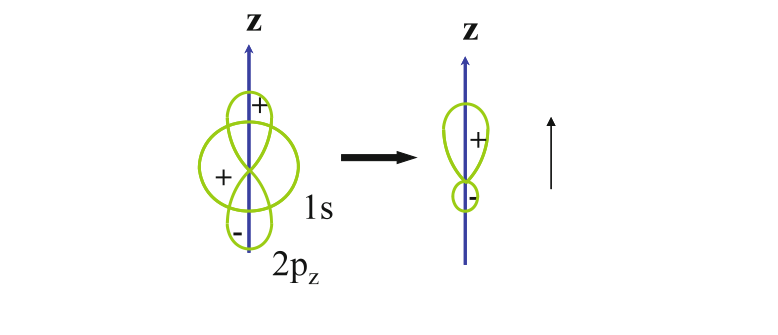
\includegraphics[width=0.8\textwidth]{images/Orbitals1s2pz.png}
    \caption{Caption}
    \label{fig:label}
\end{figure}
Dobbiamo minimizzare la funzione 
\begin{equation*}
  \mathcal{L} = \bra{a,b}H \ket{a,b} - E(a^2+b^2)
\end{equation*}
Otteniamo in questo modo l' equazione secolare
\begin{equation*}
  \det\begin{pmatrix}
    H_{11}-E & H_{12}\\
    H_{21} &H_{22}-E
  \end{pmatrix} = 0
\end{equation*}
Prendeno il livello energetico più basso si ottiene che 
\begin{equation*}
  E = E_{1s}^0+\frac{4}{3}\frac{A^2}{E_{1s}^0} = E_{1s}^0-2.96 \frac{a_0^3}{2}\mathcal{E}^2
\end{equation*}
che implica che il valore stimato di $\alpha$ è 
\begin{equation*}
  \alpha_{1s}\simeq 2.96a_0^3
\end{equation*}

\input{sections/HamiltonianInMagneticField}




% Se vuoi un blocco "Soluzione" pulito senza pacchetti extra:
\subsection*{Soluzioni (opzionale)}
% Scrivi qui, oppure commenta questa sezione.  

% --------------------
\section{Formulario e tabella delle notazioni}
% Elenco definizioni rapide, formule ricorrenti, simboli.

% --------------------
\appendix
\section{Appendice: dimostrazioni tecniche}
\section{Appendice: identità utili}
\section{Funzioni degli orbitali dell' atomo di Idrogeno}
Definendo il raggio di Bohr come 
\begin{equation*}
  a_0 = \frac{\hbar}{\alpha mc}
\end{equation*}
la parte radiale delle funzioni d' onda dei livelli dell' atomo di idrogeno sono
\begin{align*}
  R_{10} =& 2 \left(\frac{Z}{a_0}\right)^\frac{3}{2}\exp\left\{-\frac{Zr}{a_0}\right\}\\
  R_{21} =& \frac{1}{\sqrt{3}} \left(\frac{Z}{2a_0}\right)^\frac{3}{2} \left(\frac{Zr}{a_0}\right)\exp\left\{-\frac{Zr}{2a_0}\right\}\\
  R_{20} =& 2\left(\frac{Z}{2a_0}\right)^\frac{3}{2} \left(1-\frac{Zr}{2a_0}\right)\exp\left\{-\frac{Zr}{2a_0}\right\}\\
R_{32}=&\frac{2 \sqrt{2}}{27 \sqrt{5}}\left(\frac{Z}{3 a_0}\right)^{\frac{3}{2}}\left(\frac{Z r}{a_0}\right)^2 \exp\left\{-\frac{Z r}{ 3 a_0}\right\}
\end{align*}

% --------------------
\section*{Bibliografia essenziale}
% Puoi sostituire con biblatex/bibtex se vuoi.
\begin{itemize}
  \item Testo 1...
  \item Testo 2...
\end{itemize}


\subsection{Orbital and Spin magnetic moments and Spin-Orbit Interaction}
sezione che devo fare




\end{document}
